\documentclass{article}

% Language setting
% Replace `english' with e.g. `spanish' to change the document language
\usepackage[spanish]{babel}

% Set page size and margins
% Replace `letterpaper' with `a4paper' for UK/EU standard size
\usepackage[letterpaper,top=2cm,bottom=2cm,left=3cm,right=3cm,marginparwidth=1.75cm]{geometry}

% Useful packages
\usepackage{amsmath}
\usepackage{graphicx}
\usepackage{enumitem}
\usepackage{comment}
\usepackage{wrapfig}
\usepackage[colorlinks=true, allcolors=blue]{hyperref}

\title{POO Tema 7. Excepciones}
\author{Martín González Dios 
\href{https://github.com/martindios}{\includegraphics[height=0.5cm]{github.png}}}

\begin{document}
\maketitle

Una de las tareas importantes que es necesario realizar en el desarrollo de un programa es la \textbf{gestión de los errores} que ocurren durante su ejecución, ya que su correcto tratamiento facilita la usabilidad y mantenimiento del programa. Se busca \textbf{separar la lógica de la gestión de errores} con la lógica restante. \\

\begin{wrapfigure}[]{r}{0.3\linewidth}
    \centering
    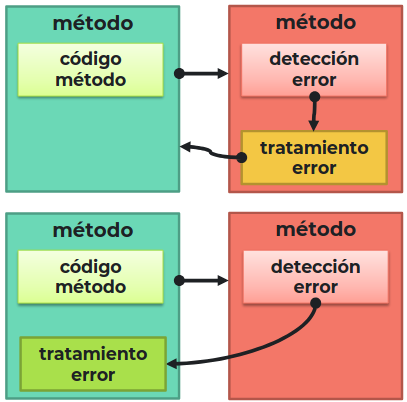
\includegraphics[width=\linewidth]{img-t7/img_439_15.png}
    \caption{Comparación de metodologías para la gestión de errores}
\end{wrapfigure}

Parte 1 (arriba). La detección y el tratamiento del error \textbf{están mezclados} con el código del método rojo, haciéndolo mucho más complejo entender y mantener. 
El método verde únicamente se encarga de invocar al método rojo.

Parte 2 (abajo). La detección del error forma parte del código del método rojo, pero es
una \textbf{parte muy pequeña del código}, lo que simplifica el método si lo comparamos con la versión (1).
El método verde mezcla el código de tratamiento del error con su código. \\

En el código método rojo se mantiene la detección del error para sacar ventaja de la simplificación en su código en relación a la versión (1).
El tratamiento del error continua en el código del método verde, pero \textbf{existe una clara separación} entre el código de tratamiento del error y el código que proporciona la funcionalidad del método verde. De este modo, un cambio en uno de los dos tipos de código \textbf{no afectaría al otro}. \\

Una \textbf{excepción} es la ocurrencia de errores y/o situaciones de interés durante la ejecución de los métodos que proporcionan la funcionalidad del programa. También se relacionan con situaciones a las que se debe dar respuesta y no solo errores. \\

El mecanismo de Java para el tratamiento de las excepciones aplica la filosofía de \textbf{separar el código} para la detección, la comunicación y el tratamiento de las excepciones del código de los métodos que proporciona la funcionalidad del programa.

\begin{figure}[h]
    \centering
    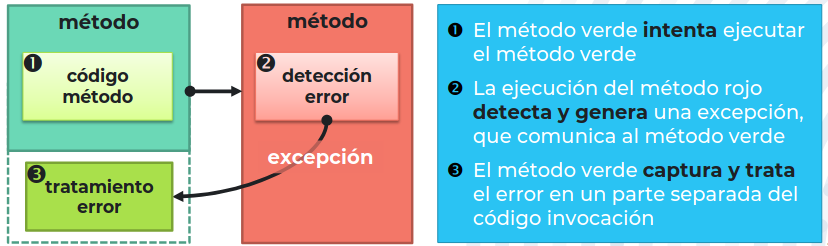
\includegraphics[width=0.65\textwidth]{img-t7/img_793_12.png}
    \caption{Tratamiento de excepciones en Java}
\end{figure}

\section{Definición de excepciones}
Antes de especificar las etapas correspondientes a la gestión de las excepciones en tiempo de ejecución es necesario (1) definir qué excepciones pueden tener lugar; y (2) definir en
qué métodos ocurrirán dichas excepciones. \\

Una excepción se especifica como una clase derivada de la \textbf{clase Throwable}, cuyos métodos más usados habitualmente son los siguientes: 
\begin{itemize}
    \item \textbf{String getMessage()} devuelve el mensaje que se ha indicado en la ocurrencia de la excepción.
    \item \textbf{void printStackTrace()} imprime en consola la secuencia de invocaciones de métodos que ha llevado a la ocurrencia de la excepción.
\end{itemize}

En \textbf{Java existen 2 tipos de excepciones}:
\begin{itemize}
    \item \textbf{Excepciones chequeadas (“checked”)}, se comprueba en tiempo de compilación en qué métodos puede ocurrir una excepción, en cuyo caso \textbf{esos métodos deben indicar de forma explícita} esa posible ocurrencia. Son \textbf{clases derivadas de la clase Exception}.
    
    \item \textbf{Excepciones no chequeadas (“uncheked”)}, no se comprueba en tiempo de compilación cuáles son los métodos en los que tiene lugar la ocurrencia de la excepción, descargando en el \textbf{programador la responsabilidad de revisar} dónde puede ocurrir para intentar capturarla y tratarla. Son \textbf{clases derivadas de las clases RuntimeException o Error}.
\end{itemize}

\begin{figure}[h]
    \centering
    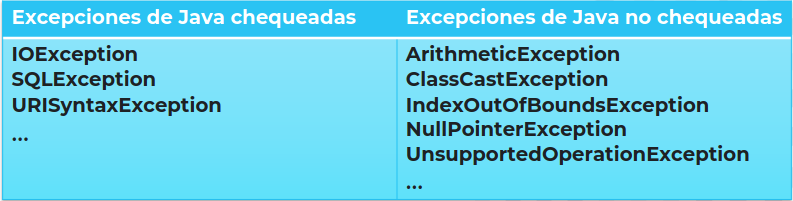
\includegraphics[width=0.75\textwidth]{img-t7/img_823_21.png}
    \caption{Ejemplos de excepciones checkeadas y no checkeadas}
\end{figure}

Si el error o la condición que ha provocado la ocurrencia de la excepción \textbf{no impide} la ejecución del programa, la excepción \textbf{debería ser del tipo chequeada}. (Ejemplo: NullPointerException es no chequeada porque en pocas ocasiones se puede ”arreglar” un nulo de un objeto). \\

\newpage

La definición de excepciones como \textbf{clases derivadas de la clase Exception} confiere a los programadores un mayor control sobre la gestión de dichas excepciones, puesto que obliga a que los métodos declaren qué excepciones podrían ocurrir durante su invocación. \\


(\textbf{public Exception(String mensaje)}) message es el mensaje con el que típicamente el programador explica por qué ha tenido lugar la ocurrencia de la excepción, que es el momento en el que se crea el objeto de tipo clase derivada de Exception. Este mensaje es lo que habitualmente se le muestra al usuario. Este constructor \textbf{debería ser invocado} desde el constructor de la clase derivada de Exception.

\begin{figure}[h]
    \centering
    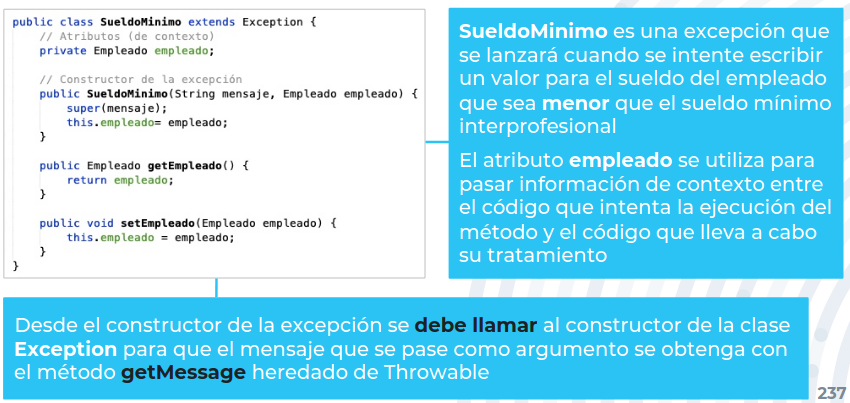
\includegraphics[width=0.9\textwidth]{img-t7/img_747_39.png}
    \caption{Ejemplo de manejo de excepciones}
\end{figure}

Para las \textbf{excepciones chequeadas}, el compilador exige que se indiquen \textbf{explícitamente} los métodos en los que tienen lugar dichas excepciones.
\begin{itemize}
    \item Se deben \textbf{etiquetar} los métodos en los que tienen lugar las excepciones.
    \item Un mismo método puede estar etiquetado \textbf{con más de un tipo de excepción}, es decir, con más de una clase derivada de Exception.
    \item Un \textbf{constructor también puede generar excepciones}.
\end{itemize}
$<tipo\_acceso>$ $<tipo\_dato>$ nombre$\_$método($<args>$ *) throws $<excepcion>$ \\
$<tipo\_acceso>$ nombre$\_$clase($<args>$ *) throws $<excepcion>$
(En la signatura del método se deberán de indicar todas las excepciones)

\newpage

\section{Gestión de excepciones: intentar}

\begin{wrapfigure}[]{r}{0.3\linewidth}
    \centering
    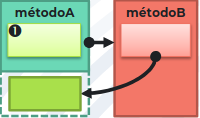
\includegraphics[width=\linewidth]{img-t7/img_604_04.png}
    \caption{El número 1 indica cuál es la parte $"Intentar"$ en la gestión de excepciones}
\end{wrapfigure}

La gestión de las excepciones comienza con la invocación de un métodoA desde otro métodoB, de modo que se puede decir que el \textbf{métodoA intenta ejecutar con éxito el métodoB}. Es necesario indicar en \textbf{qué parte del código del métodoA se va intentar la ejecución con éxito del métodoB}, es decir, se intenta la invocación del métodoB esperando obtener el resultado por el cual tiene lugar dicha invocación. \\
\textbf{try}: en el bloque try se deberá de invocar obligatoriamente al métodoB, aunque lo más deseable es que todo el código funcional del métodoA se sitúe dentro de un único bloque try para que sea más legible. \\

En el código de un puede haber \textbf{tantos bloques try como invocaciones a métodos que generan una excepción}, incluso aunque sean varias invocaciones a un mismo método.

\begin{figure}[h]
    \centering
    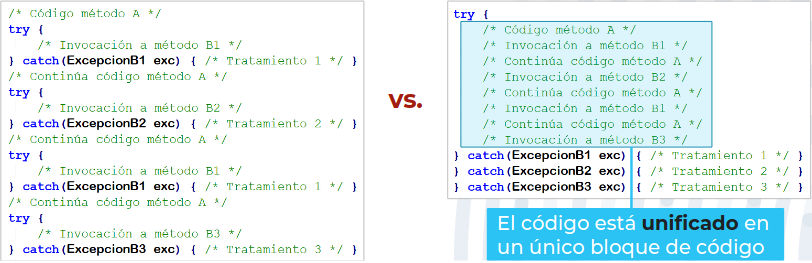
\includegraphics[width=0.85\textwidth]{img-t7/img_054_09.png}
    \caption{Ejemplo de 2 implementaciones distintas con try}
\end{figure}

\section{Gestión de excepciones: lanzar}

\begin{wrapfigure}[]{r}{0.3\linewidth}
    \centering
    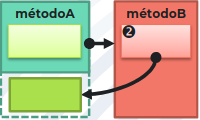
\includegraphics[width=\linewidth]{img-t7/img_118_00.png}
    \caption{El número 2 indica cuál es la parte $"Lanzar"$ en la gestión de excepciones}
\end{wrapfigure}

Una vez se invoca la ejecución del métodoB, el control del programa pasa al código de dicho
método, que tiene dos partes: (1) \textbf{la detección} y (2) \textbf{la generación} de la excepción para que sea tratada en el método que realizó la invocación.
\begin{itemize}
    \item La detección de la excepción consiste en especificar dentro del código del métodoB las \textbf{condiciones} en las cuales se genera la excepción. (Si el numerador de la división es 0)
    
    \item Al generar la excepción se completa lo que se entiende por \textbf{lanzar la excepción}, que consiste en crear un objeto del tipo de excepción que se transferirá al trozo de código en el cual tiene lugar el tratamiento de la excepción. \textbf{Cuando se crea el objeto del tipo excepción}, es habitual \textbf{incluir en ella información} sobre el contexto en el que ha ocurrido, incluyendo (a) una descripción textual sobre la causa que la ha provocado; y/o (b) referencias a objetos que se podrán usar en el tratamiento de la excepción. \\
    Al lanzar una excepción se interrumpe la ejecución del método en el mismo punto en el cual se ha lanzado, es decir, el flujo de programa abandona el método y apunta directamente al código en el que se lleva a cabo el tratamiento de la excepción.
\end{itemize}

\newpage

\begin{figure}[h]
    \centering
    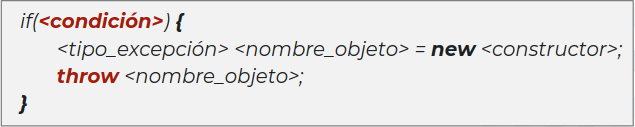
\includegraphics[width=0.65\textwidth]{img-t7/img_029_46.png}
    \caption{Uso de la palabra throw}
\end{figure}

La palabra \textbf{throw} se utiliza para indicar que se interrumpe la ejecución del método y se lanza la excepción para que pueda ser capturada por el código en el que se trata la excepción, que es el \textbf{punto en el que continúa} la ejecución del programa. \\
La información del contexto de ocurrencia de la excepción \textbf{se pasa en los argumentos del constructor} de la clase asociada a la excepción.

\begin{figure}[h]
    \centering
    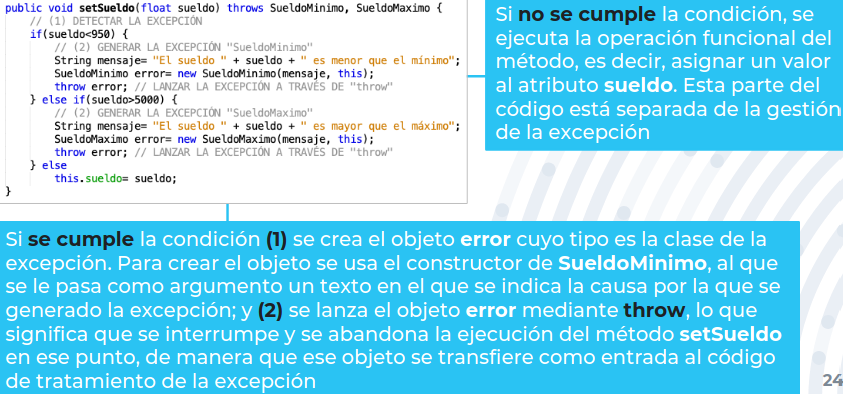
\includegraphics[width=0.95\textwidth]{img-t7/img_984_51.png}
    \caption{Ejemplo de throw}
\end{figure}

\section{Gestión de excepciones: tratar}

\begin{wrapfigure}[]{r}{0.3\linewidth}
    \centering
    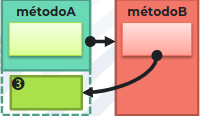
\includegraphics[width=\linewidth]{img-t7/img_953_39.png}
    \caption{El número 3 indica cuál es la parte $"Tratar"$ en la gestión de excepciones}
\end{wrapfigure}

Una vez se lanza una excepción, el objeto de tipo excepción se transfiere \textbf{como “argumento”} al código en el que se realiza su tratamiento, de modo que dicho código tiene información contextual sobre la ocurrencia de la excepción. \\
El momento en el que el flujo de programa entra en el código para el tratamiento de la excepción se denomina \textbf{captura de la excepción}. El tratamiento de la excepción tiene lugar en los denominados \textbf{bloques catch}, los cuales \textbf{no pueden existir} sin haber especificado previamente un bloque try. \\

\newpage

\textbf{Restricciones entre los bloques try-catch}:

\begin{itemize}
    \item Si existe un bloque catch deberá existir necesariamente \textbf{un único bloque try}.
    \item Un bloque try deberá tener asociado, \textbf{al menos}, un bloque catch.
    \item Un bloque try \textbf{podría tener tantos} bloques catch como el número
    de tipos de excepciones se puedan lanzar en el bloque try.
    \item Un bloque try \textbf{podría tener menos} bloques catch que el número
    de excepciones que se hayan lanzado en el bloque try. (Si las excepciones que se lanzan tienen la misma clase base, entonces puede definirse \textbf{un único bloque catch}) (Si el tratamiento es el mismo puede usarse \textbf{multi-catch})
\end{itemize}

La \textbf{opción multi-catch} no añaden ningún tipo de semántica a la gestión de la excepción, sino que está orientada a simplificar el código del bloque catch.

\begin{figure}[h]
    \centering
    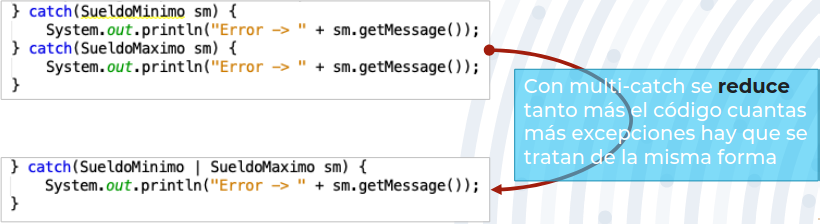
\includegraphics[width=0.75\textwidth]{img-t7/img_752_17.png}
    \caption{Ejemplo de multi-catch}
\end{figure}

Es importante el papel de la \textbf{herencia y el polimorfismo} a la hora de decidir qué bloque catch se ejecutará cuando se lanza una excepción. Si el argumento del bloque catch es una de las clases superiores a una claseA, después de ese catch \textbf{no podrá existir} un catch con la claseA, puesto que la excepción se habrá capturado en el catch de la clase superior. \\

En el tratamiento de las excepciones, además de los bloques catch también existe el \textbf{bloque finally}, que se ejecuta siempre; independientemente de la excepción que se haya capturado o incluso aunque no se haya capturado ninguna excepción.
\begin{itemize}
    \item Un bloque try puede tener asociado un \textbf{único bloque finally}.
    \item El bloque finally siempre \textbf{deberá ir después} de todos los bloques catch asociados al tratamiento de la excepción.
    \item No es posible definir un bloque finally si no existe, \textbf{al menos}, un bloque catch el que se capturen las excepciones generadas en el bloque try.
    \item Uno de los usos habituales del bloque finally \textbf{es liberar recursos}.
\end{itemize}

\newpage

\section{Como gestionar la generación de excepciones}
Un métodoA que invoca a un métodoB que lanza una excepción \textbf{no debe tener necesariamente un try–catch} como parte de su código, es decir, el métodoA no tiene por qué realizar la captura de la excepción. \textbf{El métodoA puede delegar el tratamiento de la excepción a otro métodoC que lo invoque}, de modo que existe un encadenamiento lanzamientos de excepciones que tiene como fin la unificación del código en el cual se realizar el tratamiento final de la excepción.

\begin{figure}[h]
    \centering
    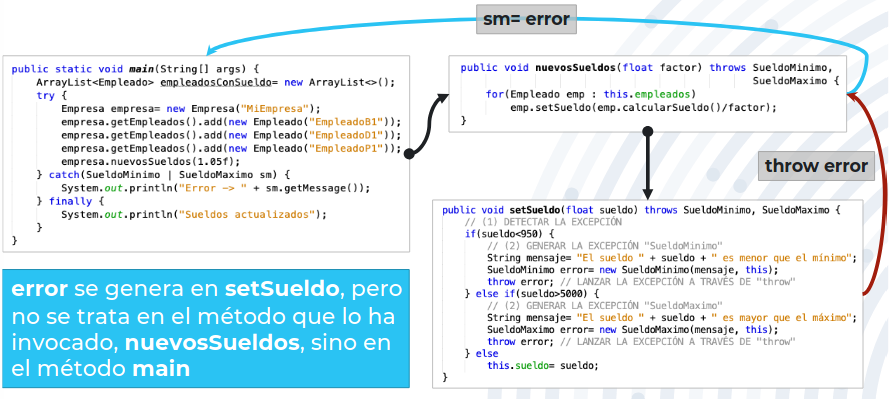
\includegraphics[width=\textwidth]{img-t7/img_737_29.png}
    \caption{Ejemplo de generación de excepciones estructurado}
\end{figure}




\begin{comment}
\begin{figure}[h]
    \centering
    \includegraphics[width=0.65\textwidth]{1.png}
    \caption{}
\end{figure}
\end{comment}

\begin{comment}
\begin{wrapfigure}[]{r}{0.45\linewidth}
    \centering
    \includegraphics[width=0.8\linewidth]{8.png}
    \caption{}
\end{wrapfigure}
\end{comment}

\end{document}